% !TEX root = ../meca1321-synthesis.tex

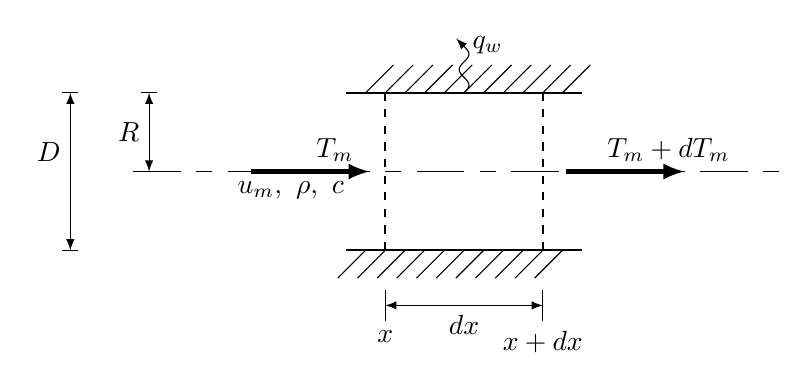
\begin{tikzpicture}
  % Tracé des parois
  \draw [thick] (-1.5,1) -- (1.5,1);
  \draw [thick] (-1.5,-1) -- (1.5,-1);
  \foreach \i in {0,...,10}
  {
    \pgfmathsetmacro{\x}{(- 1.5 + \i/4)};
    \draw (\x+1/4,1) -- ++(45:0.5);
    \draw (\x+1/4,-1) -- ++(-135:0.5);
  }
  %Repères et autres flèches
  \draw [>=latex,<->] (-5,-1) -- (-5,1);
  \draw (-4.1,1) -- ++(0.2,0);
  \draw (-4,0.5) node [left] {$R$};
  \draw [>=latex,<->] (-4,0) -- (-4,1);
  \draw (-5.1,1) -- ++(0.2,0);
  \draw (-5.1,-1) -- ++(0.2,0);
  \draw (-5,0) node [above left] {$D$};
  \draw [dash pattern= on 0.6cm off 0.2cm on 0.2cm off 0.2cm] (-4.2,0) -- (4,0);
  \draw [ultra thick,>=latex,->] (-2.7,0) -- ++(1.5,0);
  \draw [thick, dashed] (-1, -1) -- (-1, 1);
  \draw [thick, dashed] (1, -1) -- (1, 1);
  \draw [ultra thick,>=latex,->] (1.3, 0) -- ++(1.5,0);
  \draw (3.5, 0) node [above left] {$T_m + dT_m$};
  \draw (-2, 0) node [above right] {$T_m$};
  \draw (-3, 0) node [below right] {$u_m,~\rho,~c$};
  \draw (-1, -1.5) -- ++(0, -0.4) node [below] {$x$};
  \draw (1, -1.5) -- ++(0, -0.4) node [below] {$x+dx$};
  \draw [>=latex,<->] (-1, -1.7) -- ++(2, 0);
  \draw (0, -1.7) node [below] {$dx$};
  \draw [domain=0:3*pi] plot ({sin(deg(\x))/16}, {\x/16+1}) [>=latex, ->] -- ++(-0.1,0.1);
  \draw (0.3, 1.6) node {$q_w$};
\end{tikzpicture}
